%%%%%%%%%%%%%%%%%%%%%%%%%%%%%%%%

\documentclass[11pt,a4paper]{article}
\usepackage{times}
\usepackage[utf8]{inputenc}
\usepackage[croatian]{babel}
\usepackage[T1]{fontenc} % Latin Modern

%%%%%%%%%%%%%%%%%%%%%%%%%%%%%%%%


%%%%%%%%%%%%%%%%%%%%%%%%%%%%%%%%
%%%%%%%%  MATEMATICKI PAKETI %%%%%%%%%%%
%%%%%%%%%%%%%%%%%%%%%%%%%%%%%%%%

\usepackage{amsmath}
\usepackage{amsfonts}
\usepackage{amssymb}
\usepackage{esvect}

%%%%%%%%%%%%%%%%%%%%%%%%%%%%%%%%

%%%%%%%%%%%%%%%%%%%%%%%%%%%%%%%%
%%%%%%%%%% PAKETI ZA SLIKE  %%%%%%%%%%%%
%%%%%%%%%%%%%%%%%%%%%%%%%%%%%%%%

\usepackage{graphicx}
\usepackage{float}
\usepackage[hidelinks]{hyperref}
\usepackage{caption}
\usepackage{subcaption}
\usepackage{booktabs}

%%%%%%%%%%%%%%%%%%%%%%%%%%%%%%%%

%%%%%%%%%%%%%%%%%%%%%%%%%%%%%%%%
%%%%%%%%%    PRORED 1.5   %%%%%%%%%%%%%%
%%%%%%%%%%%%%%%%%%%%%%%%%%%%%%%%

\renewcommand{\baselinestretch}{1.5}

%%%%%%%%%%%%%%%%%%%%%%%%%%%%%%%%


%%%%%%%%%%%%%%%%%%%%%%%%%%%%%%%%
%%%%%%%%%% TABLICA - ANTUN %%%%%%%%%%%%
%%%%%%%%%%%%%%%%%%%%%%%%%%%%%%%%

\usepackage{array}
\usepackage{multirow}
\newcolumntype{C}[1]{>{\centering\let\newline\\\arraybackslash\hspace{0pt}}m{#1}}
\newcolumntype{L}[1]{>{\raggedright\let\newline\\\arraybackslash\hspace{0pt}}m{#1}}
\newcolumntype{R}[1]{>{\raggedleft\let\newline\\\arraybackslash\hspace{0pt}}m{#1}}
\usepackage{ctable}

%%%%%%%%%%%%%%%%%%%%%%%%%%%%%%%%

%%%%%%%%%%%%%%%%%%%%%%%%%%%%%%%%
%%%%%%%%%% TABLICA - MARTINA %%%%%%%%%%%
%%%%%%%%%%%%%%%%%%%%%%%%%%%%%%%%

\makeatletter
\renewcommand*\env@matrix[1][\arraystretch]{%
  \edef\arraystretch{#1}%
  \hskip -\arraycolsep
  \let\@ifnextchar\new@ifnextchar
  \array{*\c@MaxMatrixCols c}}
\makeatother



%%%% LATEX KOD ZA KORISTENJE TABLICE %%%%
%%% PRIMJER %%%

%\setlength\extrarowheight{1pt}
%\begin{table}[h]
%\centering
%\caption{Tablica s prikazom }
%\label{prva}
%\begin{tabular}{|l|c|}
%\hline
%\textbf{txt} &  \\ \hline 
%txt & txt    \\ 
%txt & txt   \\ \hline
%txt & txt    \\ \hline
%\end{tabular}
%\end{table}

%%%%%%%%%%%%%%%%%%%%%%%%%%%%%%%%


%%%%%%%%%%%%%%%%%%%%%%%%%%%%%%%%
%%%%%%% DIO ZA UNOS ISJECAKA KODA %%%%%%%%
%%%%%%%%%%%%%%%%%%%%%%%%%%%%%%%%

\usepackage{listings}
\usepackage{color}
 
\definecolor{codegreen}{rgb}{0,0.6,0}
\definecolor{codegray}{rgb}{0.5,0.5,0.5}
\definecolor{codepurple}{rgb}{0.58,0,0.82}
 
\lstdefinestyle{mystyle}{   
    commentstyle=\color{codegreen},
    keywordstyle=\color{blue},
    numberstyle=\tiny\color{codegray},
    stringstyle=\color{codepurple},
    basicstyle=\footnotesize,
    breakatwhitespace=false,         
    breaklines=true,                 
    captionpos=b,                    
    keepspaces=true,                 
    numbers=left,                    
    numbersep=5pt,                  
    showspaces=false,                
    showstringspaces=false,
    showtabs=false,                  
    tabsize=1
}
 
\lstset{style=mystyle}

%\lstinputlisting[language=Matlab, firstline=1, lastline=4, numbers=left, frame=single, label={lst:prvi}, caption={Diskretizacija sustava korištenjem Matlaba}, captionpos=b]{peti.m} 

%%%%%%%%%%%%%%%%%%%%%%%%%%%%%%%%


%----------------------------
% za uredjenje stranice
\usepackage[left=2.5cm,right=2.5cm,top=2.5cm,bottom=2.5cm]{geometry}
\usepackage{fancyhdr}
\pagestyle{fancy} 
\lhead{\leftmark}
\rhead{\rightmark}
\usepackage{titlesec} %za točku iza broja sectiona
\titleformat{\section}{\huge\bfseries}{\thetitle.\quad}{0em}{}
\titleformat{\subsection}{\LARGE\bfseries}{\thetitle.\quad}{0em}{}
\titleformat{\subsubsection}{\Large\bfseries}{\thetitle.\quad}{0em}{}
\titleformat{\paragraph}
{\normalfont\large\bfseries}{\thetitle.\quad}{1em}{}
\titlespacing*{\paragraph}
{0pt}{3.25ex plus 1ex minus .2ex}{1.5ex plus .2ex}
\setcounter{secnumdepth}{5}

\usepackage{indentfirst} %uvlacenje prvog paragrafa
% primjer pozivanja sectiona
% \section*{UVOD} \pdfbookmark{UVOD}{section:UVOD}

\usepackage{tocloft}
\usepackage{import}
\usepackage{standalone}
\graphicspath{{Uvod/}, {Ciljevi/}, {Materijal/}, {Rasprava/}, {Rezultati/}} 

\hypersetup{
  colorlinks   = true, %Colours links instead of ugly boxes
  urlcolor     = black, %Colour for external hyperlinks
  linkcolor    = black, %Colour of internal links
  citecolor   = blue %Colour of citations
}

\usepackage{subcaption}
\usepackage{lscape}
\begin{document}

POGLAVLJE NAZVATI ELEKTRONIČKO SLOPOVLJE

U ovom poglavlju je predstavljen dizajn i izrada elektroničkog sklopovlja potrebnog za upravljanje multirotorskom letjelicom s pomičnim masama. Elektroničko sklopovlje je ciljano dizajnirano za upravljanje koračnim motorima koji u ovom slučaju predstavljaju pokretne mase. Također, kao pripremu za daljnja proširenja, dodana su standarna sučelja za komunikaciju i akuatore koja se koriste u radu laboratorija. Elektroničko sklopovlje je zasnovano na mikrokontroleru STM32 serije F4. Dodatno, na elektroničkom sklopovlju trebaju postojati izvodi napajanja standardnih iznosa $3.3 V$ i $5 V$. Sklopovlje se napaja iz baterije nazivnog napona $12 V$. 

Dizajn elektroničkog sklopovlja izrađen je u CAD alatu \textit{Altium Designer}. Altium predstavlja standardni CAD alat za izradu elektroničkog sklopovlja. U okviru ovog alata, definiraju se sve potrebne elektroničke komponente, s pripadnim fizičkim rasporedom veza i mogućnošću dodavanja 3D modela svake pojedine komponente. Prvo se pristupa projektiranju sklopovlja na shematskoj razini. U ovom koraku definiraju se sve sheme, određuju se komponente koje je kasnije potrebno kupiti sa svim pripadnim podacima. Nakon završetka prve faze projektiranja, slijedi fizički raspored komponenata na tiskanu pločicu i povezivanje svih električnih veza. U obje faze projekiranja, softver omogućava kontrolu prema zadanim postavkama te na taj način upozorava korisnika ukoliko je došlo do kršenja zadanih pravila, poput kratkih spojeva, prebliskih električnih vodova i slično.

Funkcionalnost elektroničkog sklopovlja i programske potpore je provjerena izradom prototipa. Prototip je realiziran perforiranom pločicom, na koju su postavljene i povezane sve bitne komponente, prvenstveno pogoni koračnih motora. Upravljanje pogonima koračnih motora omogućeno je razvojnom pločicom \textit{STM Discovery}, baziranom na STM32 mikrokontroleru serije F4, koji je korišten i u konačnom posebno prilagođenom sklopovlju.



\begin{figure}[H]
	\centering
	\includegraphics[width=0.6\textwidth]{figures/arducopter_pcb.png}
	\caption{3D model elektroničkog sklopovlja}
	\label{Slika:3D_PCB}
\end{figure}

\subsection{Sastavni dijelovi elektroničkog slopovlja}

\subsubsection{Napajanje}
Napajanje elektroničkog sklopovlja je osigurano baterijom nazivnog napona 12 V. Na ulazu napajanja dodan je osigurač iznosa 10 A. Iznos osigurača je projektiran prema snazi koračnih motora i \textit{Dynamixel} motora. U sklopu modula napajanja, potrebno je osigurati stabilne iznose napona 3.3 V i 5V. Prva razina spuštanja ulaznog napona je osigurana 5V regulatorom napona, switching tipa. Specifikacije regulatora su prikazane tablicom \ref{tab:specifikacija_5V}.


\begin{table}[H]
	\centering
	\caption{Specifikacije 5V regulatora napona}
	\label{tab:specifikacija_5V}
	\begin{tabular}{|l|c|}
		\hline
		\textbf{Proizvođač} & Texas instuments  \\ \hline 
		\textbf{Model} &  LM2592HVS-5.0  \\ \hline 
		\textbf{Tip} &  Buck(Step Down) Switching Regulator  \\ \hline 
		\textbf{Minimalni ulazni napon} & 4.5 V \\ \hline 
		\textbf{Maksimalni ulazni napon} & 60 V \\ \hline 
		\textbf{Izlazni napon} & 5 V \\ \hline 
		\textbf{Izlazna struja} & 2 A \\ \hline 
		\textbf{Frekvencija rada} & 150 kHz \\ \hline 
		\textbf{Maksimalna radna temperatura} & $125 ^\circ C$ \\ \hline 
	\end{tabular}
\end{table}

Nadalje, napon iznosa 3.3 V osiguran je snižavanjem napona iznosa 5V iz prethodno opisanog regulatora. U ovom slučaju korišten je linearni regulator. Korištenje ovog tipa regulatora je moguće, budući da je snaga potrošača spojenih na napajanje 3.3 V daleko manja od maksimalnog iznosa struje koju daje 5 V regulator. Specifikacije 3.3 V regulatora prikazane su tablicom \ref{tab:specifikacija_3V3}

\begin{table}[H]
	\centering
	\caption{Specifikacije 3.3V regulatora napona}
	\label{tab:specifikacija_3V3}
	\begin{tabular}{|l|c|}
		\hline
		\textbf{Proizvođač} & ST Microelectronics \\ \hline 
		\textbf{Model} &  LD1117S33TR \\ \hline 
		\textbf{Tip} &  Fixed LDO Voltage Regulator  \\ \hline 
		\textbf{Minimalni ulazni napon} & 4.75 V \\ \hline 
		\textbf{Maksimalni ulazni napon} & 15 V \\ \hline 
		\textbf{Izlazni napon} & 3.3 V \\ \hline 
		\textbf{Izlazna struja} & 800 mA \\ \hline 
		\textbf{Maksimalna radna temperatura} & $125 ^\circ C$ \\ \hline 
	\end{tabular}
\end{table}

U sklopu modula napajanja, potrebno je osigurati i napajanje koračnih motora te napajanje Dynamixel motora. U ovom slučaju, koristi se ulazni napon, međutim dodani su jumperi, kako bi na jednostavan način bilo moguće odspojiti navedene potrošače u fazi programiranja elektroničkog sklopovlja.

\subsubsection{Mikrokontroler}
 Elektroničko sklopovlje je bazirano na mikrokontroleru \textit{STM32}, serije F4. Jezgra mikrokontrolera je zasnovana na jezgri \textit{ ARM$\textregistered$ Cortex$^{TM}$ - M4}, 32-bit, RISC arhitekture. Na mikrokontroler su povezane sve komponente kojima je potrebno upravljati i s kojih je potrebno očitavati stanja. Specifikacije mikrokontrolera su prikazane tablicom \ref{tab:specifikacija_MCU}.

\begin{table}[H]
	\centering
	\caption{Specifikacije STM mikrokontrolera}
	\label{tab:specifikacija_MCU}
	\begin{tabular}{|l|c|}
		\hline
		\textbf{Proizvođač} & ST Microelectronics \\ \hline 
		\textbf{Model} &  STM32F405RGT6V \\ \hline 
		\textbf{Jezgra} & \textit{ ARM$\textregistered$ Cortex$^{TM}$ - M4}, 32-bit, RISC  \\ \hline 
		\textbf{CPU brzina} & 168 MHz \\ \hline 
		\textbf{Veličina RAM memorije} & 192 KB \\ \hline 
		\textbf{Broj pinova} & 64 \\ \hline 
		\textbf{Broj I/O jedinica} & 51 \\ \hline 
		\textbf{Ugrađena sučelja} & CAN, I2C, SPI, UART, USART, USB\\ \hline 
		\textbf{Minimalni napon napajanja} & 1.8 V\\ \hline 
		\textbf{Maksimalni napon napajanja} & 3.6 V\\ \hline 
	\end{tabular}
\end{table}

Napajanje mikrokontrolera je osigurano reguliranim naponom iznosa 3.3V. Dodatno stabiliziranje napona je osigurano dodavanjem kondenzatora različitih iznosa. Dodatni kondenzatori su smješteni u neposrednoj blizini mikrokontrolera na tiskanoj pločici. Kao izvor takta mikrokontrolera korišten je kristalni oscilator nazivne frekvencije 8 Mhz.

\subsubsection{LED indikatori}
Prilikom izrade prototipa elektroničkog sklopovlja utvrđena je potreba postojanja LED indikatora. LED indikatori se koriste u svrhu provjere ispravnosti rada programske potpore. U ovom slučaju, dodane su 4 LED diode različitih boja. LED diode su spojene na mikorokontroler, a za izvor napajanja se koristi regulirani napon iznosa 5V. Upravljanje LED diodama je ostvareno mikrokontrolerom i bipolarnim NPN tranzistorom. Struja koja protječe LED diodom prilikom visoke razine upravljačkog signala iz mikrokontrolera je ograničena dodavanjem otpornika iznosa 500 Ohm. 


\subsubsection{Pogon koračnih motora}

Pogon koračnih motora ostvaren je gotovim sklopom \textit{A4988}. Navedeni sklop ima sadržano upravljanje naponima i strujama svake faze koračnog motora. Pogonski sklop predstavlja međusklop između koračnog motora i mikroprocesora. Mikroprocesor postavljanjem logičkih razina na predviđene pinove upravlja smjerom vrtnje i rezolucijom koraka. Kretanje motora se izvodi generiranjem impulsnog signala. Generiranje impulsnog signala je ostvareno prikladnom programskom potporom mikrokontrolera. Specifikacije sklopa \textit{A4988} prikazane su tablicom \ref{tab:specifikacija_stepper_driver}.


\begin{figure}[H]
	\centering
	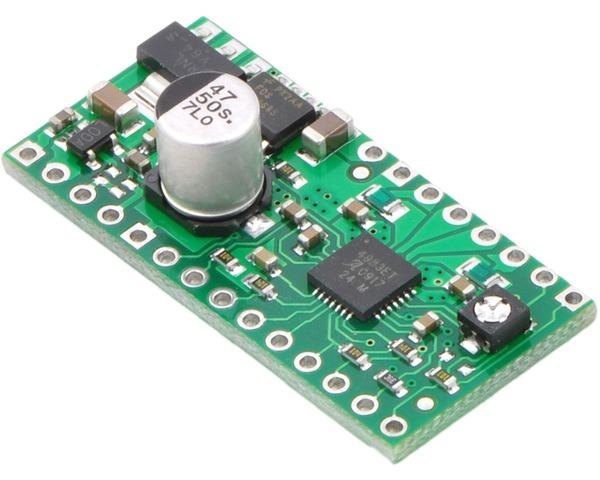
\includegraphics[width=0.4\textwidth]{figures/driver.jpg}
	\caption{Prikaz pogona koračnog motora}
	\label{Slika:stepper_driver}
\end{figure}

Sklop \textit{A4988} se napaja izravno s baterije, a napajanje logike je ostvareno korištenjem ugrađenih regulatora napona u samom sklopu. Mikrokontroler upravlja radom pogonskog sklopa pomoću 5 pinova:
\begin{center}
	\begin{itemize}
		\item \textit{STP} - impulsni signal broja koraka
		\item \textit{DIR} - smjer vrtnje motora
		\item \textit{MS1} - upravljanje rezolucijom koraka
		\item \textit{MS2} - upravljanje rezolucijom koraka
		\item \textit{MS3} - upravljanje rezolucijom koraka
	\end{itemize}
\end{center}


\begin{table}[H]
	\centering
	\caption{Specifikacije pogona koračnih motora}
	\label{tab:specifikacija_stepper_driver}
	\begin{tabular}{|l|c|}
		\hline
		\textbf{Proizvođač} & Pololu \\ \hline 
		\textbf{Model} & A4988 \\ \hline 
		\textbf{Veličina} &  17.78mm x 35.56mm  \\ \hline 
		\textbf{Masa} & 3.3 g \\ \hline 
		\textbf{Minimalni ulazni napon} & 8 V \\ \hline 
		\textbf{Maksimalni ulazni napon} & 35 V \\ \hline 
		\textbf{Kontinuirana stuja po fazi} & 1 A, bez hladnjaka \\ \hline 
		\textbf{Maksimalna struja po fazi} & 2 A, s hladnjakom \\ \hline 
		\textbf{Minimalni napon logike} & 3 V\\ \hline 
		\textbf{Maksimalni napon logike} & 5.5 V\\ \hline 
		\textbf{Rezolucija mikrokoraka} & puni korak, 1/2, 1/4, 1/8 i 1/16\\ \hline 
		\textbf{Zaštita obrnutog polariteta} & Da\\ \hline 
	\end{tabular}
\end{table}


\subsubsection{Konektori}

Za ispravno i sigurno povezivanje elektroničkog sklopovlja s okolnim uređajima potrebno je ispravno odabrati konektore. Konektori korišteni na ovom elektroničkom sklopu su:
\begin{center}
	\begin{itemize}
		\item Konektor za DC napajanje, kutni. Navedeni konektor se koristi za spajanje elektroničkog sklopovlja na izvor napajanja. Specifikacije konektora zadovoljavaju navedenu primjenu, a prikazane su tablicom \ref{tab:specifikacija_supply_connector}.
		
\begin{table}[H]
	\centering
	\caption{Specifikacije konektora DC napajanja}
	\label{tab:specifikacija_supply_connector}
	\begin{tabular}{|l|c|}
		\hline
		\textbf{Proizvođač} & Molex \\ \hline 
		\textbf{Model} & 172310-1102 \\ \hline 
		\textbf{Dobavljač} & Farnell \\ \hline 
		\textbf{Broj pinova} & 2 \\ \hline 
		\textbf{Način motaže} & Trough hole    \\ \hline
		\textbf{Pitch} & 3.50 mm    \\ \hline 
		\textbf{Maksimalni napon} & 400 V \\ \hline 
		\textbf{Maksimalna struja} & 14 A \\ \hline
		\textbf{Otpor izolacije} & 100 MOhm \\ \hline
	\end{tabular}
\end{table}		
		
		\item Konektor za programiranje mikrokontrolera. Spajanjem specijalnog programatora na ovaj konektor, izvodi se programiranje mikrokontrolera.
		
		\item Konektor za serijsku vezu, korišten za upravljanje koračnim motorima. Navedeni tip konektora se koristi i na kontroleru leta Pixhawk. Zbog svog dizajna, kontroler je otporan na vibracije, što je izrazito bitno za primjenu na letjelici. Specifikacije konektora su prikazane tablicom \ref{tab:specifikacija_connector_serial}.
		
\begin{table}[H]
	\centering
	\caption{Specifikacije konektora serijske veze}
	\label{tab:specifikacija_connector_serial}
	\begin{tabular}{|l|c|}
		\hline
		\textbf{Proizvođač} & JST \\ \hline 
		\textbf{Serija proizvoda} & GH \\ \hline 
		\textbf{Dobavljač} & RS \\ \hline 
		\textbf{Broj pinova} & 3 \\ \hline 
		\textbf{Način motaže} & Surface Mount    \\ \hline
		\textbf{Pitch} & 1.25 mm    \\ \hline 
		\textbf{Maksimalni napon} & 50 V  ac/dc\\ \hline 
		\textbf{Maksimalna struja} & 1 A \\ \hline
	\end{tabular}
\end{table}		

		
		\item Konektor za \textit{Dynamixel} motor. Zbog paralelnog načina spajanja motora, jedan konektor na programskom sklopovlju je dovoljan za upravljanje s više \textit{Dynamixel} motora. Konektor koji se nalazi na ovom sklopovlju je identičan konektoru na \textit{Dynamixel} motoru. Specifikacije konektora su prikazane tablicom \ref{tab:specifikacija_connector_dynamixel}.
		
\begin{table}[H]
	\centering
	\caption{Specifikacije konektora Dynamixel motora}
	\label{tab:specifikacija_connector_dynamixel}
	\begin{tabular}{|l|c|}
		\hline
		\textbf{Proizvođač} & Molex \\ \hline 
		\textbf{Serija proizvoda} & SPOX 5267 \\ \hline 
		\textbf{Dobavljač} & Farnell \\ \hline 
		\textbf{Broj pinova} & 3 \\ \hline 
		\textbf{Način motaže} & Trough Hole    \\ \hline
		\textbf{Pitch} & 2.5 mm    \\ \hline 
		\textbf{Maksimalni napon} & 250 V \\ \hline 
		\textbf{Maksimalna struja} & 3 A \\ \hline
	\end{tabular}
\end{table}
		
		\item Konektori za spajanje faza koračnih motora. Upravljanje naponima faza koračnih motora se ostvaruje pomoću 4 žice, dvije po fazi. Budući da na koračnim motorima ne postoji poseban konektor, odabran je jednostavni konektor u koji se žice faza koračnih motora fiksiraju pomoću vijka.
		
\begin{table}[H]
	\centering
	\caption{Specifikacije blok konektor za spajanje koračnih motora}
	\label{tab:specifikacija_connector_terminal}
	\begin{tabular}{|l|c|}
		\hline
		\textbf{Proizvođač} & Phoenix Contact \\ \hline 
		\textbf{Serija proizvoda} & MPT \\ \hline 
		\textbf{Dobavljač} & Farnell \\ \hline 
		\textbf{Broj pinova} & 4 \\ \hline 
		\textbf{Način motaže} & Trough Hole    \\ \hline
		\textbf{Pitch} & 2.54 mm    \\ \hline 
		\textbf{Površina vodiča, CSA} & 0.5 mm$^2$     \\ \hline 
		\textbf{Maksimalni napon} & 125 V \\ \hline 
		\textbf{Maksimalna struja} & 6 A \\ \hline
	\end{tabular}
\end{table}
		
		
		\item Konektor za CAN komunikaciju. Navedeni konektor sadrži potrebne kontakte za napajanje i dvije podatkovne linije. Konektor je iste serije kao i konektor za serijsku vezu, osnovna razlika je u broju pinova. Specifikacije konektora za CAN komunikaciju su prikazane tablicom \ref{tab:specifikacija_connector_CAN}.
		
\begin{table}[H]
	\centering
	\caption{Specifikacije konektora CAN komunikacije}
	\label{tab:specifikacija_connector_CAN}
	\begin{tabular}{|l|c|}
		\hline
		\textbf{Proizvođač} & JST \\ \hline 
		\textbf{Serija proizvoda} & GH \\ \hline 
		\textbf{Dobavljač} & RS \\ \hline 
		\textbf{Broj pinova} & 4 \\ \hline 
		\textbf{Način motaže} & Surface Mount    \\ \hline
		\textbf{Pitch} & 1.25 mm    \\ \hline 
		\textbf{Maksimalni napon} & 50 V  ac/dc\\ \hline 
		\textbf{Maksimalna struja} & 1 A \\ \hline
	\end{tabular}
\end{table}
		
		
		\item Konektor za slobodne pinove. Na elektroničkom slopovlju postoje izvodi svih naponski razina kao i 5 izravnih spojeva na GPIO izlaze mikrokontrolera. Namjena ovog konektora je omogućiti buduće modifikacije i proširenja funkcionalnosti.	
		
	\end{itemize}
\end{center}



\subsubsection{Dynamixel}
Upravljanje Dynamixel motorima ostvaruje se prikladnom elektroničkom i programskom potporom. Osnova elektroničkog sklopovlja za Dynamixel komunikaciju je sklop za dvosmjernu komunikaciju. Mikrokontroler upravlja sklopom za dvosmjernu komunikaciju, koristeći 3 signala: \textit{DYN\_SEL}(odabir smjera komunikacije), \textit{DYN\_RX}(primanje podatka s Dynamixel motora) i \textit{DYN\_TX}(slanje podatka na Dynamixel motore). NAPISATI ČEMU SLUŽI HRPA OTPORNIKA I TRANZISTORA!!! Uz Dynamixel komunikaciju, potrebno je dodati i napajanje. Napajanje je izravno s baterije, a stabilizacija napona je ostvarena kondenzatorom iznosa 220 uF. Kondenzator se na tiskanoj pločici nalazi neposredno pored konektora za Dynamixel.

\begin{table}[H]
	\centering
	\caption{Specifikacije sklopa za dvosmjernu komunikaciju}
	\label{tab:specifikacija_dynamixel_buffer}
	\begin{tabular}{|l|c|}
		\hline
		\textbf{Proizvođač} & Texas Instuments \\ \hline 
		\textbf{Model} & SN74LVC2G241DCTR \\ \hline 
		\textbf{Način montaže} & Surface Mount, SSOP-8 \\ \hline 
		\textbf{Broj pinova} & 8 \\ \hline 
		\textbf{Minimalni napon napajanja} & 1.65 V \\ \hline 
		\textbf{Maksimalni napon napajanja} & 5.5 V    \\ \hline
	\end{tabular}
\end{table}


\subsubsection{CAN}
Fizički sloj CAN komunikacije je ostvaren primjenom posebnog sklopa za CAN komunikaciju. Specifikacije sklopa su prikazane tablicom \ref{tab:specifikacija_CAN_bus}. Naveni sklop zadovoljava standard norme ISO 11898-2, za fizički sloj CAN komunikacije visoke brzine. Napajanje sklopa je ostvareno korištenjem reguliranog napona 3.3V, uz dodavanje dodatnih kondenzatora za stabilizaciju napona. Kondenzatori su na tiskanoj pločici postavljeni neposredno pored sklopa. Mikrokontroler upravlja primanjem i slanjem podataka pomoću dva signala(\textit{DRV\_IN} - slanje, \textit{DRV\_OUT} - primanje). Izlaz iz sklopa su dvije CAN linije, visoke i niske razine. Refleksije na kraju linije su spriječene dodavanjem otpornika iznosa 120 Ohm.

\begin{table}[H]
	\centering
	\caption{Specifikacije sklopa za CAN komunikaciju}
	\label{tab:specifikacija_CAN_bus}
	\begin{tabular}{|l|c|}
		\hline
		\textbf{Proizvođač} & Texas Instuments \\ \hline 
		\textbf{Model} &  SN65HVD232D \\ \hline 
		\textbf{Način montaže} & Surface Mount, SOIC \\ \hline 
		\textbf{Broj pinova} & 8 \\ \hline 
		\textbf{Minimalni napon napajanja} & 3 V \\ \hline 
		\textbf{Maksimalni napon napajanja} & 3.6 V    \\ \hline
	\end{tabular}
\end{table}

\subsection{Tiskana pločica - PCB}

\subsubsection{Projektiranje tiskane pločice}
Nakon izrade shema elektroničkog sklopovlja slijedi projektiranje tiskane pločice. Tiskana pločica je dvoslojna, a dimenzija je identična dimenziji osnovne ploče smještene na tijelu letjelice. Projektiranje tiskane pločice se obavlja također u \textit{Altium Designer} CAD alatu. U nastavku slijedi kratki pregled procesa projektiranja tiskane pločice:

\begin{center}
	\begin{enumerate}
		\item \textbf{Definiranje oblika, veličine pločice i broja slojeva.} Pločica je kvadratnog oblika, dimenzija 116mm x 116mm i sadrži 2 sloja bakra.
		
		\item \textbf{Raspored komponenata.} Na gornjoj strani pločice smješteni su svi konektori, pogoni koračnih motora, regulatori napona, LED diode, mikrokontoler i kristalni oscilator. Preostale komponente nalaze se na doljnjem sloju pločice. Prilikom rapospoređivanja komponenata bitno je voditi računa o načinu spajanja svake komponente prema ostatku komponenata na sklopovlju. Na taj način se olakšava slijedeći korak, fizičko povezivanje komponenata bakrenim vodovima.
		\item \textbf{Povezivanje komponenata bakrenim vodovima.} U ovom koraku bitno je ispravno definirati širinu pojedinih vodova, ovisno o očekivanom maksimalnom iznosu struje u vodiču. Širina bakrenih vodova prikazana je tablicom \ref{tab:specifikacija_pcb_with}.

\begin{table}[H]
	\centering
	\caption{Specifikacije širina bakrenih vodova na tiskanoj pločici}
	\label{tab:specifikacija_pcb_with}
	\begin{tabular}{|c|c|c|c|}
			\hline 
		  					& \textbf{Min [mil]} 	& \textbf{Preporučeno [mil]}	& \textbf{Max [mil]} \\ \hline  \hline
		 Ulazno napajanje 	& 50 	& \textbf{100} 			& 200 \\ \hline
		 Napajanje pogona koračnih motora 	& 100 	& \textbf{100} 			& 200 \\ \hline
		 Faze koračnih motora 	& 100 	& \textbf{100} 			& 200 \\ \hline
		 Napajanje Dynamixel motora 	& 25 	& \textbf{80} 			& 80 \\ \hline
		 Regulirani napon 5V 	& 25 	& \textbf{25} 			& 50 \\ \hline
		 Regulirani napon 3.3V 	& 10 	& \textbf{25} 			& 25 \\ \hline
		 Signalni vodovi 	& 10 	& \textbf{25}			& 25 \\ \hline
	\end{tabular}
\end{table}		

		\item \textbf{Povezivanje pinova mase, GND.} Doljnji sloj tiskane pločice koristi se kao sloj mase, što znači da su sve paznine koje postoje ispunjene bakrom i kratko spojene na masu. Na ovaj način osigurana je ispravna i stabilna masa elektroničkog sklopovlja.
		\item \textbf{Automatska programska kontrola rasporeda komponenata i vodova opcijom \textit{Altium Designer} alata.} CAD alat omogućava provjeru ispravnosti dizajnirane tiskane pločice na način da provjerava zadane kriterije poput, kratkih sojeva, međusobne udaljenosti vodova, širine klasa vodova i slično.
	\end{enumerate}
\end{center}


\subsubsection{Izrada i montaža tiskane pločice}
Nakon završetka dizajna tiskane pločice, projekt napravljen u CAD alatu \textit{Altium Designer} je poslan na izradu u firmu specijaliziranu za izradu tiskanih pločica.  Nakon završetka izrade, izvršit će se završna montaža, tj. lemljenje komponenata na tiskanu pločicu. Nakon montaže komponenata, slijedi faza programiranja sklopovlja i provjere ispravnosti.


\end{document}